\documentclass[12pt,letterpaper,english,bibliography=totocnumbered, abstract=on]{scrartcl}

\usepackage{indentfirst}
\usepackage[titletoc]{appendix}
\usepackage{fullpage}
%\usepackage{subfiles}
\usepackage[T1]{fontenc}
\usepackage[latin9]{inputenc}
\usepackage{color}
\usepackage{babel}
\usepackage{verbatim}

\usepackage{listings}
%\lstset{
%	basicstyle=\small\ttfamily,
%	columns=flexible,
%	breaklines=true
%}

\usepackage[unicode=true,pdfusetitle,
bookmarks=true,bookmarksnumbered=false,bookmarksopen=false,
breaklinks=true,pdfborder={0 0 0},pdfborderstyle={},backref=false,colorlinks=true]
{hyperref}
\hypersetup{linkcolor=blue,citecolor=blue,urlcolor=blue}

\usepackage{booktabs}
\usepackage{multirow}
\usepackage{adjustbox}
\usepackage{threeparttable}
\usepackage[table]{xcolor}
\usepackage{csquotes}
\usepackage{soul} % for hiliting text: \hl

\usepackage[backend=biber, style=authoryear, maxbibnames=99, dashed=false]{biblatex}
\setlength\bibitemsep{2\itemsep}
%\addbibresource{mylibrary.bib}
%\addbibresource{CRB.bib}

\usepackage{pdfpages}
\usepackage{float} % Allows use of H to place floats

\usepackage{pgfgantt}

\usepackage{framed}

% Prevent page breaks within paragraphs
% https://tex.stackexchange.com/questions/21983/how-to-avoid-page-breaks-inside-paragraphs
\widowpenalties 1 10000

\begin{document}

\titlehead{Technical Report}

\title{Monitoring Cycad Aulacaspis Scale (CAS), \textit{Aulacaspis yasumatsui}, Infesting \textit{Cycas micronesica} in the Tinian Conservation Plots using Sticky Traps}

\author{Aubrey Moore and Jason Andrew}

\date{
	April 2, 2022, Revised April 7, 2022
	\footnote{
		The most recent version of this document may be downloaded from \url{https://github.com/aubreymoore/Tinian-CAS/raw/main/reports/sticky_traps.pdf}.
		
		All data and code used in this report are available in a public GitHub repository at
		\url{https://github.com/aubreymoore/Tinian-CAS}.
	}
}

\maketitle
%\footnote{\url{https://github.com/aubreymoore/2020-FS-CRB-biocontrol-project/blob/master/combined-proposal.pdf}}


\begin{abstract}
\item
Visual examination of sticky traps yielded no indication of the presence of biocontrol agents for CAS. This corroborates examination of leaf samples which also indicated no biocontrol activity. Introduction of the predaceous lady beetle, \textit{Rhyzobius lophanthae}, from Rota should be considered.
Visual examination of sticky traps found scale crawlers on only 9 of the 24 traps even though the scale infestation covered all plots. Visual examination of the sticky traps indicated presence of only a few predaceous lady beetles and none of these could readily be associated with CAS.
Partially because of time constraints, sticky traps were deployed for only one day. Results suggest that sampling over a few days, possibly as long as one week, would be preferable for monitoring.

\end{abstract}



\clearpage
\tableofcontents

\clearpage
\section{Methods}

\paragraph{Traps.} Traps were constructed by placing pieces of yellow sticky trap material (Alpha Scents Inc., Portland, Oregon; \href{https://www.alphascents.com/large-10x16-sticky-rectangle-card-trap.html}{LGSTKYCARD}) into four-inch square polystyrene Petri dishes (Carolina Biological Supply Company, Burlington, North Carolina; \href{https://www.carolina.com/lab-dishes/polystyrene-square-integrid-petri-dish-pack-of-10/741470.pr}{Item No. 741470}). Traps were deployed in the cycad conservation plots on Tinian on 2022-02-25 and picked up on 2022-02-26. Each trap was fixed at a height of 1 meter to a stake placed 1 meter downwind (south-east) from a \textit{Cycas micronesica} plant. One trap was placed within each of the 24 plots. When traps were retrieved, Petri dish tops were secured with rubber bands and they were placed in a freezer prior to transport to Guam. Level of scale insect infestation on the nearest cycad was recorded using a 3-level categorical scale (Low, Medium, High).

Coordinates for the traps were not recorded. However, plot identification numbers were recorded. Plot centroids were calculated, using the QGIS \textbf{Mean coordinate(s)} tool, from a shapefile named \textbf{dissolvetrial} extracted from the project GIS database and these were used to approximate trap locations. For the plot numbered 14, the midpoint between plot 141 and 142 was used.

Raw data were stored in a text file, \textbf{mean\_coordinates.csv} (\ref{rawdata}). A Jupyter notebook, \textbf{pairwise-correlations.ipynb}, was created to perform pairwise correlation analysis for level of scale infestation, presence of trapped crawlers and presence of trapped coccinellids.

\paragraph{Rapid scan.} Each trap was scanned under a dissecting microscope to assess presence or absence of scale crawlers, adult male scales, predatory lady beetles (coccinellids), and parasitoids.

\paragraph{Digital image analysis.} In progress. This document will be updated when digital image analysis is complete.



\section{Results}

\begin{itemize}

\item
Field observation rated the level of scale insect infestation as high in 18 plots, medium in 5 plots and low in 1 plot (Fig. \ref{fig:scalelevel}).

\item
Scale crawlers were trapped in 9 of the 24 plots (Fig. \ref{fig:crawlers}).

\item
Coccinellids were trapped in 3 of the 24 plots (Fig. \ref{fig:coccinellids}). There is no reason to associate any of these with \textit{A. yasumatsui}. None of these appear to be \textit{Rhyzobius lophanthae}, the coccinellid purposefully introduced on Guam and Rota as a biocontrol agent for \textit{A. yasumatsui}.

\item
Male scale insects were not seen in any of the traps.

\item
A diversity of insect parasitoids were seen in the traps. There is no reason to associate any of these with \textit{A. yasumatsui}.

\item
Pairwise correlation analysis for level of scale infestation, presence of trapped crawlers and presence of trapped coccinellids shows no correlation (Fig. \ref{fig:heatmap}).

\end{itemize}


\begin{figure}[p]
	\centering
	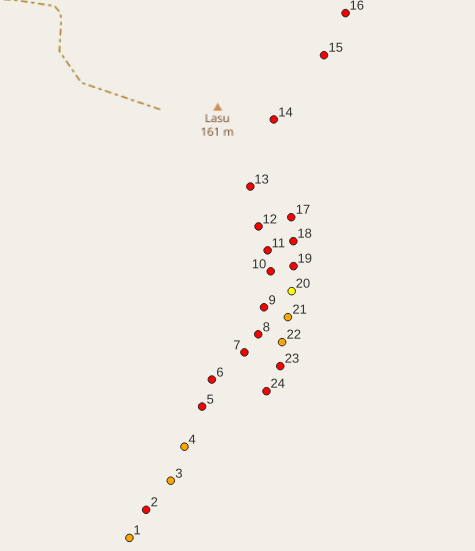
\includegraphics[width=\linewidth]{../sticky_traps/scale_level}
	\caption{Field evaluation of CAS infestation level. Yellow: Low, Orange: Medium, Red: High.}
	\label{fig:scalelevel}
\end{figure}

\begin{figure}[p]
	\centering
	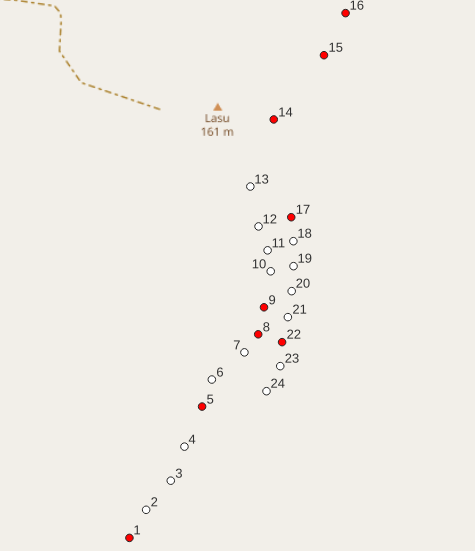
\includegraphics[width=\linewidth]{../sticky_traps/crawlers}
	\caption{Red points indicate capture of scale crawlers in sticky traps.}
	\label{fig:crawlers}
\end{figure}

\begin{figure}[p]
	\centering
	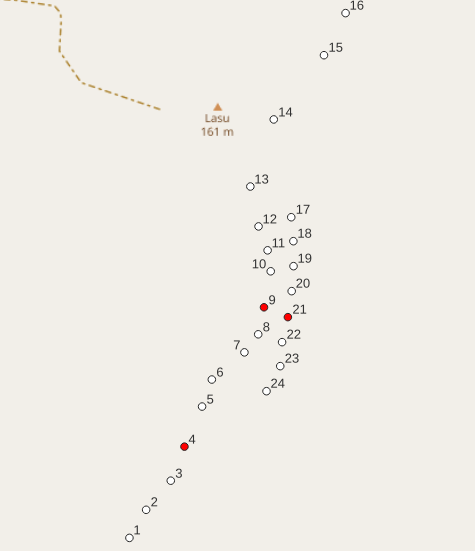
\includegraphics[width=\linewidth]{../sticky_traps/coccinellids}
	\caption{Red points indicate capture of predaceous lady beetles in sticky traps.}
	\label{fig:coccinellids}
\end{figure}

\begin{figure}[p]
	\centering
	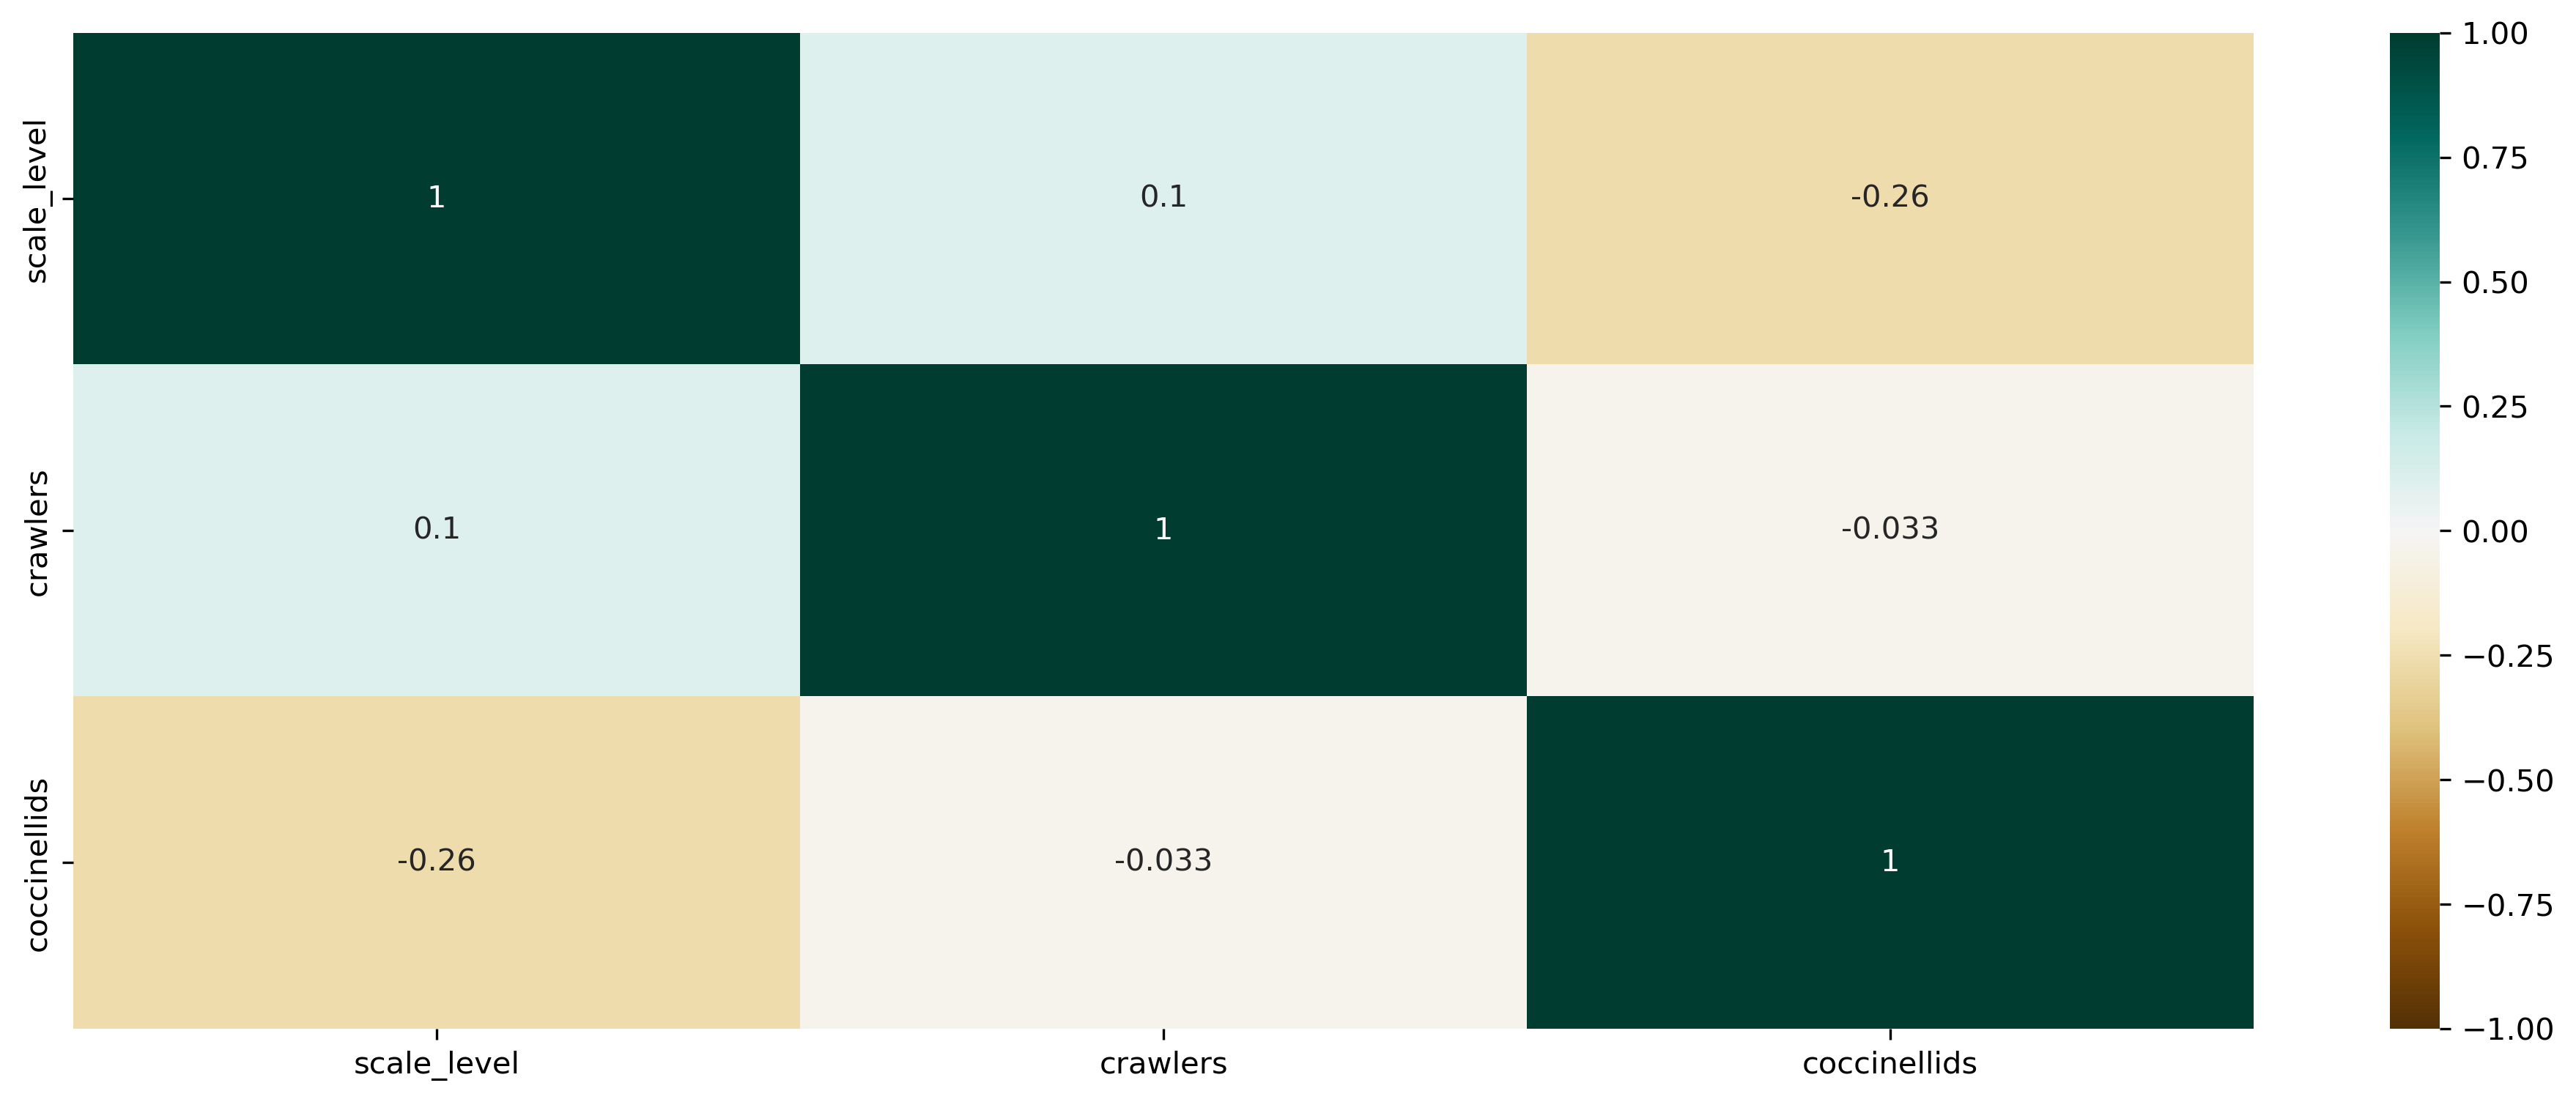
\includegraphics[width=\linewidth]{../sticky_traps/heatmap}
	\caption{Result of pairwise correlation analysis for CAS infestation level, \textbf{scale\_level}, presence of scale crawlers, \textbf{crawlers}, in traps and presence of predaceous lady beetles in traps, \textbf{coccinellids}. No significant correlation is evident.}
	\label{fig:heatmap}
\end{figure}



\section{Discussion}

\begin{itemize}

\item
Visual examination of sticky traps yielded no indication of the presence of biocontrol agents for CAS. This corroborates examination of leaf samples which also indicated no biocontrol activity. Introduction of the predaceous lady beetle, \textit{Rhyzobius lophanthae}, from Rota should be considered.

\item
Visual examination of sticky traps found scale crawlers on only 9 of the 24 traps even though the scale infestation covered all plots. Visual examination of the sticky traps indicated presence of only a few predaceous lady beetles and none of these could readily be associated with CAS.

\item
Partially because of time constraints, the sticky traps were deployed for only one day. Results suggest that sampling over a few days would be preferable for monitoring.

\end{itemize}

\clearpage
\begin{appendices}
	
	\section{Raw data: mean\_coordinates2.csv}
	\label{rawdata}
	\lstinputlisting[basicstyle=\small\ttfamily, breaklines=true, columns=flexible]{../sticky_traps/mean_coordinates2.csv}
		
	\section{Bibtex record}
	\begin{lstlisting}[basicstyle=\small\ttfamily, breaklines=true, columns=flexible]
	@misc{moore-2022-04-02,
	title = {Monitoring Cycad Aulacaspis Scale (CAS), \textit{Aulacaspis yasumatsui}, Infesting \textit{Cycas micronesica} in the Tinian Conservation Plots using Sticky Traps},
	author = {Aubrey Moore and Jason Andrew},
	url = {https://github.com/aubreymoore/Tinian-CAS/raw/main/reports/sticky_traps.pdf} 	
	}
	\end{lstlisting}
		
\end{appendices}

\end{document}
